\section{Proposed Method}
\label{sec:proposed_method}
\begin{figure*}[t]
	\begin{center}
	       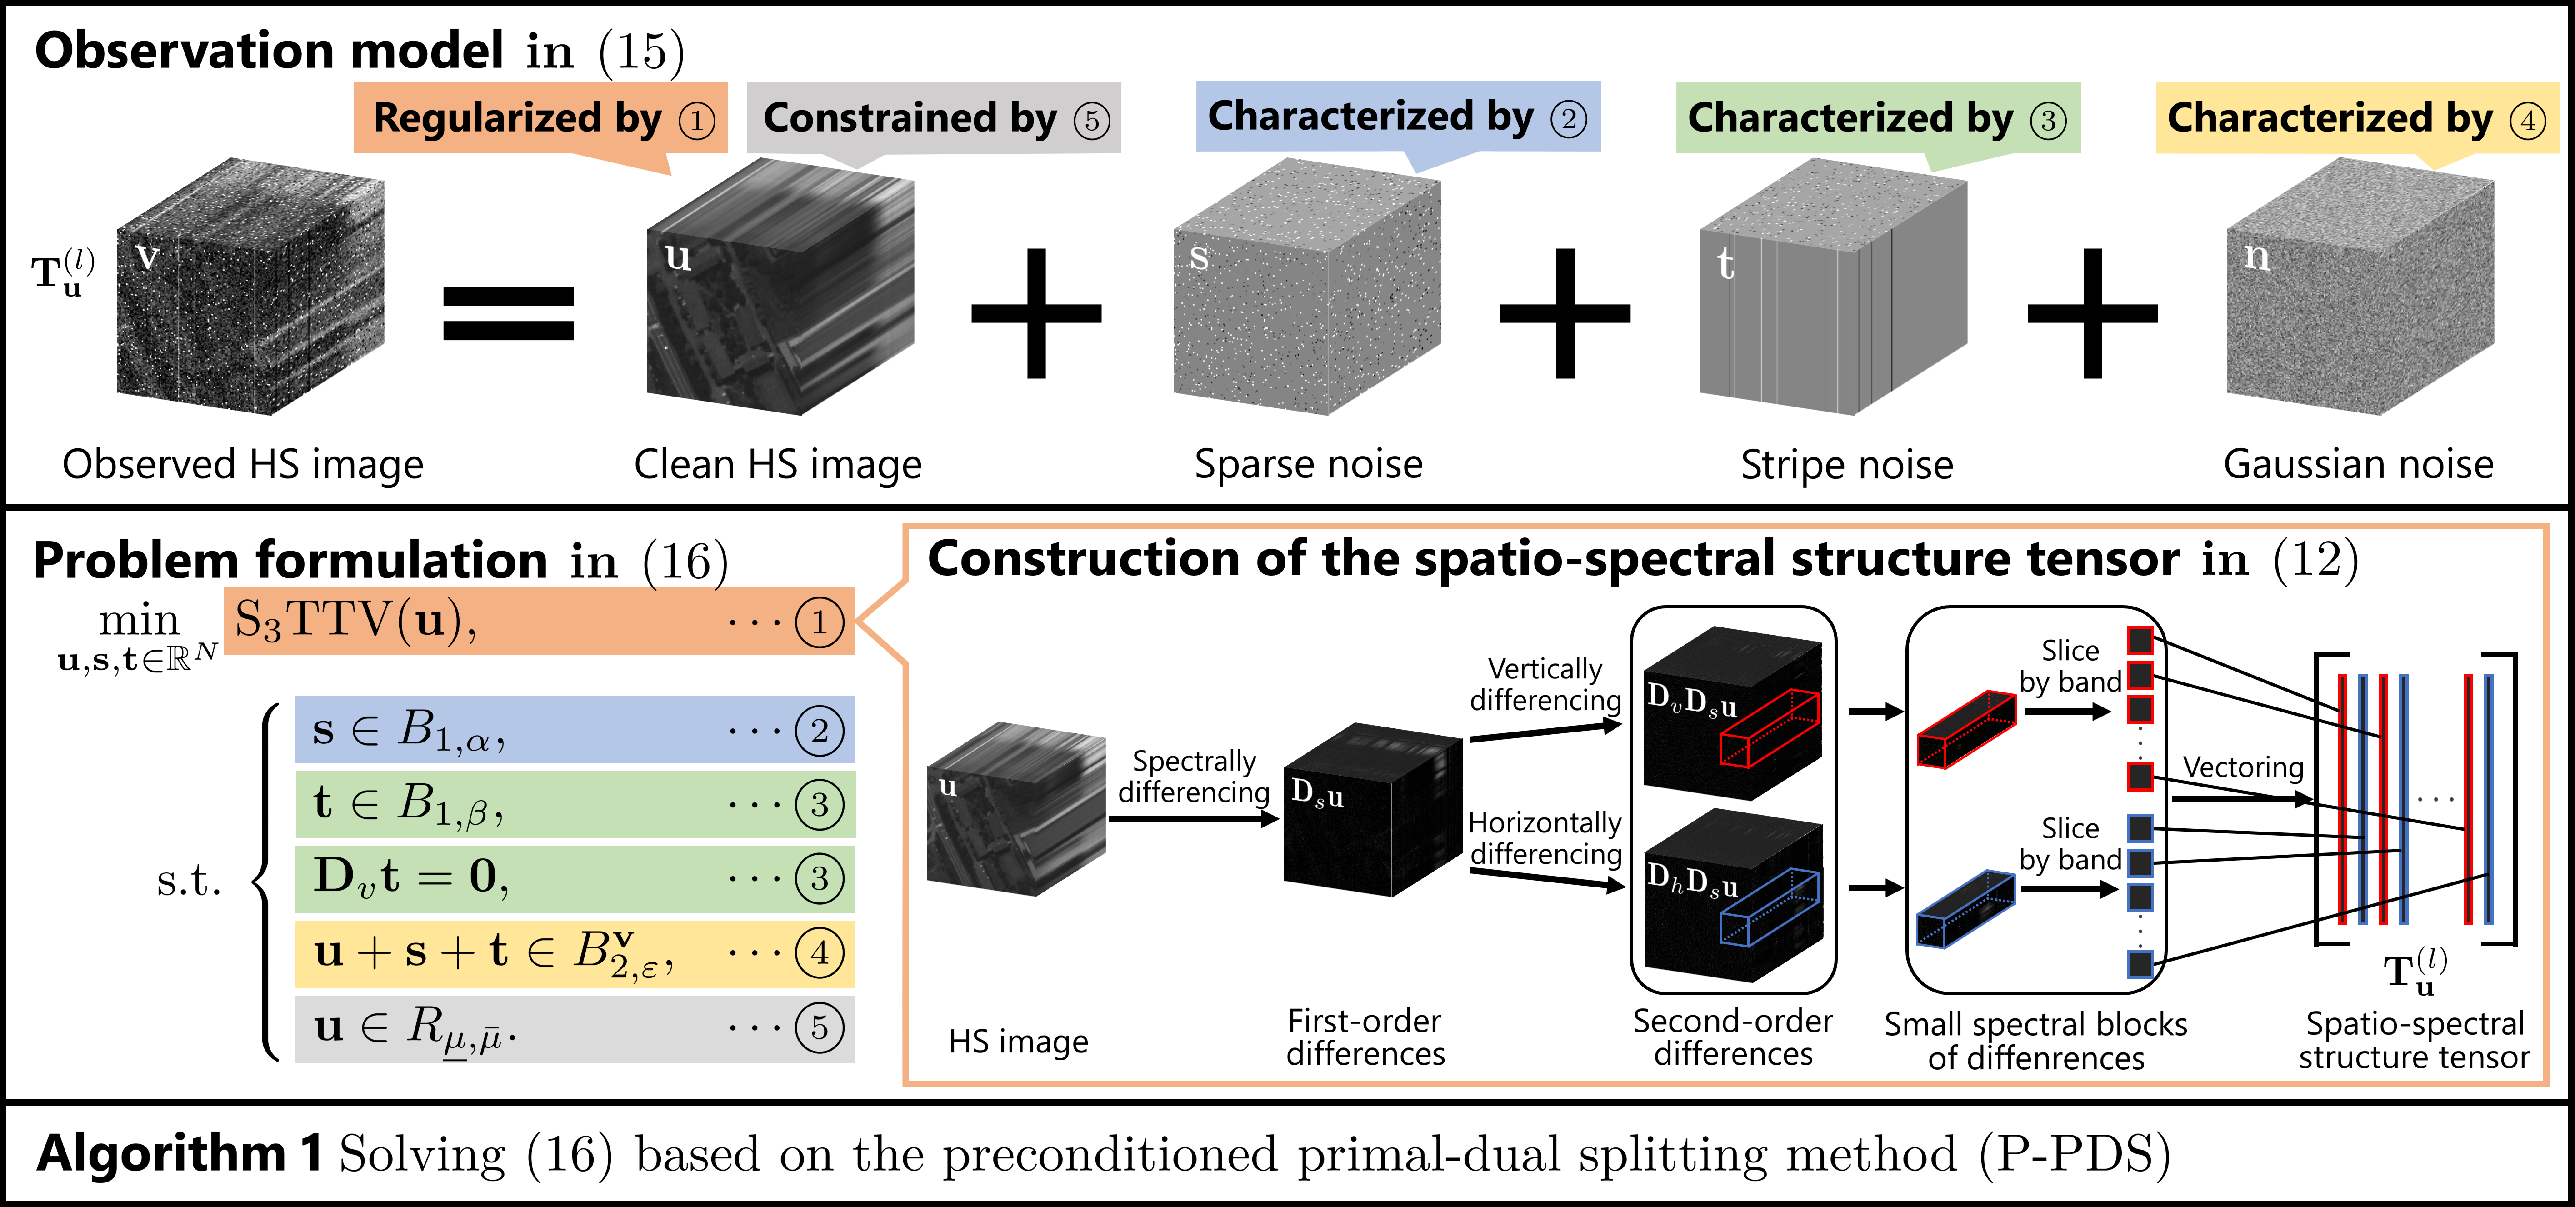
\includegraphics[width=\hsize]{./fig_supplement/Illustration_proposed_method.pdf}
	\end{center}
	\caption{Illustration of the proposed method, i.e., $\SSSTTV$.}
	\vspace{-2mm}
	\label{fig:schematic_diagram}
\end{figure*}

In the following, we first describe the design of the $\SSSTTV$ regularization function. Next, we consider a situation where an HS image is contaminated with mixed noise and introduce the corresponding observation model. Based on this model, we formulate an HS image denoising problem as a constrained convex optimization problem involving the $\SSSTTV$ regularization function. Finally, we derive an algorithm based on P-PDS to efficiently solve the optimization problem. A schematic diagram of $\SSSTTV$ is shown in Fig.~\ref{fig:schematic_diagram}.

\subsection{Spatio-Spectral Structure Tensor Total Variation ($\SSSTTV$)}
\label{subsec:S3TTV}
Before describing the proposed regularization function, we introduce the notion of \textit{spatio-spectral structure tensor}\footnote{In the SSST paper~\cite{Kurihara2017SSST}, a structure tensor with the same name as the one we proposed (i.e., spatio-spectral structure tensor) is introduced. However, they are essentially different because the structure tensor in SSST consists of first-order differences, whereas that in our regularization function consists of second-order spatio-spectral differences.}.
First, for a given HS image $\HSIClean$, we calculate the second-order spatial-spectral differences $\DiffOpVert \DiffOpBand \HSIClean$ and $\DiffOpHori \DiffOpBand \HSIClean$.
Next, we extract \textit{small spectral blocks} by cropping the second-order spatio-spectral differences to the size $\NumBlockVert \times \NumBlockHori (\NumBlockVert << \NumVert, \NumBlockHori << \NumHori)$ for all bands\footnote{At the boundaries, the block cannot be cropped to an $\NumBlockVert \times \NumBlockHori \times \NumBand$ size. For example, when the difference is cropped to a $3 \times 3 \times \NumBand$ block at a center $(1, 1)$, a $2 \times 2 \times \NumBand$ block is created. In this case, we pad the lacking areas with pixels on the opposite boundaries to make the block $\NumBlockVert \times \NumBlockHori \times \NumBand$.}. Then, the $\IndexBlock$-th spatio-spectral structure tensor $\SmallBlock{\IndexBlock}$ is defined by vectorizing the second-order spatio-spectral differences in the $\IndexBlock$-th small spectral block by band and arranging them in parallel as follows:
\begin{equation}
	\begin{split}
		\label{eq:SSST}
		\SmallBlock{\IndexBlock} :=  
		&\bigl( \lbrack \DiffOpVert \DiffOpBand \HSIClean \rbrack_{1}^{(\IndexBlock)} \: 
		\lbrack\DiffOpHori \DiffOpBand \HSIClean \rbrack_{1}^{(\IndexBlock)} \\ 
		& \: \cdots \lbrack \DiffOpVert \DiffOpBand \HSIClean \rbrack_{\NumBand}^{(\IndexBlock)} \:
		\lbrack\DiffOpHori \DiffOpBand \HSIClean \rbrack_{\NumBand}^{(\IndexBlock)} 
		\bigr) \in \RealSpace{\NumBlockVert \NumBlockHori \times 2\NumBand},
	\end{split}
\end{equation}
where $\lbrack \DiffOpVert \DiffOpBand \HSIClean \rbrack_{\IndexBand}^{(\IndexBlock)} \in \RealSpace{\NumBlockVert \NumBlockHori}$ and $\lbrack \DiffOpHori \DiffOpBand \HSIClean \rbrack_{\IndexBand}^{(\IndexBlock)} \in \RealSpace{\NumBlockVert \NumBlockHori}$ are the second-order spatio-spectral differences of $\IndexBand$-th band in the $\IndexBlock$-th small spectral block. Since HS images have the strong correlation across all bands, $\lbrack \DiffOpVert \DiffOpBand \HSIClean \rbrack_{1}^{(\IndexBlock)}, \ldots, \lbrack \DiffOpVert \DiffOpBand \HSIClean \rbrack_{\NumBand}^{(\IndexBlock)}$ and $\lbrack \DiffOpHori \DiffOpBand \HSIClean \rbrack_{1}^{(\IndexBlock)}, \ldots, \lbrack \DiffOpHori \DiffOpBand \HSIClean \rbrack_{\NumBand}^{(\IndexBlock)}$ are similar vectors, respectively, i.e., the columns of $\SmallBlock{\IndexBlock}$ are approximately linearly dependent. The flow of constructing the spatio-spectral structure tensor is depicted in the middle right of Fig.~\ref{fig:schematic_diagram}.


To capture the spatial piecewise-smoothness, the spatial similarity between adjacent bands, and the spectral correlation of an HS image, we propose a regularization function using the spatio-spectral structure tensors as follows:
\begin{equation}
	\label{eq:S3TTV_Lu}
	\textstyle \SSSTTV (\HSIClean) := \sum_{\IndexBlock=1}^{\NumBlock} \| \SmallBlock{\IndexBlock} \|_{*},
\end{equation}
where $\NumBlock$ is the number of the extracted small spectral blocks.
We call this function as \textit{Spatio-Spectral Structure Tensor Total Variation} ($\SSSTTV$).
Here, $\SmallBlock{\IndexBlock}$ is represented with an operator $\ExpantionOp{\IndexBlock} \in \RealSpace{2 \NumBlockVert \NumBlockHori \NumBand \times 2 \NumVert \NumHori \NumBand}$ that extracts the $\IndexBlock$-th small spectral block as
\begin{equation}
	\label{eq:rewrite_Lu}
	\SmallBlock{\IndexBlock}
	= \ExpantionOp{\IndexBlock} \DiffOpSp \DiffOpBand \HSIClean.
\end{equation}


Minimizing the nuclear norms of the matrices $\SmallBlock{1}, \ldots, \SmallBlock{\NumBlock}$ allows for both the reduction of the energy of second-order differences and the enhancement of the spectral correlation of second-order differences. By reducing the energy of second-order differences instead of first-order differences, the proposed method promotes both the spatial piecewise-smoothness and the spatial similarity between adjacent bands while avoiding over-smoothing, as shown in~\cite{Aggarwal2016SSTV}. Furthermore, experimental analysis also indicates that second-order differences are more effective than first-order differences in distinguishing noise from HS images (see Sec.~\ref{subsec:Discussion}-4) on p. 13 for details). On the other hand, by enhancing the spectral correlation of second-order difference, the proposed method enhances the spectral correlation of HS images (see Appendix~A on p. 16 for proof). Therefore, by solving an optimization problem that incorporates $\SSSTTV$, our method simultaneously captures the above three natures.


\subsection{HS Image Denoising Problem by $\SSSTTV$}
\label{subsec:HSI_Denoising_Problem}
An observed HS image $\HSIObsv \in \RealSpace{\NumAll}$ contaminated by mixed noise is modeled by
\begin{equation}
	\label{eq:Obsevation_model}
	\HSIObsv = \bar{\HSIClean} + \bar{\NoiseSparse} + \bar{\NoiseStripe} + \NoiseGauss,
\end{equation}
where $\bar{\HSIClean}$ is a clean HS image, $\bar{\NoiseSparse}$ is sparse noise, $\bar{\NoiseStripe}$ is stripe noise, and $\NoiseGauss$ is Gaussian noise, respectively.
Modeling different types of noise as separate components is an effective approach for mixed noise removal in HS images~\cite{Zhang2022Double}.

Based on the above observation model, we formulate an HS image denoising problem involving $\SSSTTV$ as a constrained convex optimization problem with the following form:
\begin{equation}
	\label{prob:S3TTV_denoising}
	\min_{\HSIClean, \NoiseSparse, \NoiseStripe \in \RealSpace{\NumAll}} \SSSTTV(\HSIClean) \: \mathrm{s.t.} \:
	\begin{cases} 
		\NoiseSparse \in \BallSparse, \\ 
		\NoiseStripe \in \BallStripe, \\
		\DiffOpVert \NoiseStripe = \mathbf{0}, \\
		\HSIClean + \NoiseSparse + \NoiseStripe \in \BallFidel, \\  
		\HSIClean \in \SetRange,
	\end{cases}
\end{equation}
where
\begin{align}
	\label{eq:constraint_sparse}
	&\BallSparse := \{ \VarOne \in \RealSpace{\NumAll} | \:
	\|\VarOne\|_{1} \leq \RadiusSparse \},  \\
	\label{eq:constraint_stripe}
	&\BallStripe := \{ \VarOne \in \RealSpace{\NumAll} | \:
	\|\VarOne\|_{1} \leq \RadiusStripe \},  \\
	\label{eq:constraint_fidel}
	&\BallFidel := \{ \VarOne \in \RealSpace{\NumAll} | \:
	\|\VarOne - \HSIObsv\|_2 \leq \RadiusFidel \},  \\
	\label{eq:constraint_box}
	&\SetRange := \{ \VarOne \in \RealSpace{\NumAll} | \:
	\MinRange \leq \ElementOne{\IndexOne} \leq \MaxRange  \: (\IndexOne = 1, \dots , \NumAll) \}.
\end{align}

The first constraint characterizes sparse noise $\NoiseSparse$ with the zero-centered $\ell_1$-ball of the radius $\RadiusSparse > 0$. The second constraint controls the intensity of stripe noise $\NoiseStripe$ and the third constraint captures the vertical flatness property by imposing zero to the vertical gradient of $\NoiseStripe$. These constraints effectively characterize stripe noise~\cite{Naganuma2022Destriping}. The fourth constraint serves as data-fidelity with the $\HSIObsv$-centered $\ell_2$-ball of the radius $\RadiusFidel > 0$. The fifth constraint is a box constraint with $\MinRange < \MaxRange$ which represents the dynamic range of $\HSIClean$. For normalized HS images, we can set $\MinRange = 0$ and $\MaxRange = 1$.


Using the first, second, and fourth constraints instead of adding terms to the objective function makes it much easier to adjust the parameters $\RadiusSparse$, $\RadiusStripe$, and $\RadiusFidel$. This is because by expressing multiple terms as constraints, rather than adding them to the objective function, the hyperparameters associated with each term are converted to be independent of each other, and appropriate parameters can be determined without interdependence. Such advantage has been addressed, e.g., in~\cite{Afonso2011Constraint, Chierchia2015Constraint, Ono2015Constraint, Ono2017Constraint, Ono2019Constraint}.


\subsection{Optimization}
\label{subsec:Optim}
To solving Prob.~\eqref{prob:S3TTV_denoising} by an efficient algorithm based on P-PDS~\cite{Pock2011PPDS}, we need to reformulate it into the P-PDS applicable form~\eqref{prob:convex_optim_prob}. Using the indicator functions $\FuncIndicator{\SetZero}$, $\FuncIndicator{\BallFidel}$, $\FuncIndicator{\BallStripe}$, $\FuncIndicator{\BallSparse}$, and $\FuncIndicator{\SetRange}$, we rewrite Prob.~\eqref{prob:S3TTV_denoising} into an equivalent form:
\begin{align}
	\label{prob:denoising2PPDS}
	\min_{
		\substack{
			\HSIClean, \NoiseSparse, \NoiseStripe\\ 
			\VarDualMatrix{1,1}, \ldots , \VarDualMatrix{1,\NumBlock}, 
			\VarDual{2}, \VarDual{3}}} \:
	& \sum_{\IndexBlock=1}^{\NumBlock} \| 
	\VarDualMatrix{1, \IndexBlock} \|_{*}
	+ \FuncIndicator{\SetZero} (\VarDual{2})
	+ \FuncIndicator{\BallFidel} (\VarDual{3}) \nonumber \\
	& + \FuncIndicator{\BallSparse} (\NoiseSparse) 
	+ \FuncIndicator{\BallStripe} (\NoiseStripe)
	+ \FuncIndicator{\SetRange} (\HSIClean),  \nonumber \\
	& \mathrm{s.t.} \:
	\begin{cases} 
		\VarDualMatrix{1,1} = \ExpantionOp{1} \DiffOpSp \DiffOpBand \HSIClean, \\ 
		\vdots \\ 
		\VarDualMatrix{1,\NumBlock} = \ExpantionOp{\NumBlock} \DiffOpSp \DiffOpBand \HSIClean, \\ 
		\VarDual{2} = \DiffOpVert \NoiseStripe, \\
		\VarDual{3} = \HSIClean + \NoiseSparse + \NoiseStripe. 
	\end{cases}
\end{align}
Let $\HSIClean$, $\NoiseSparse$, and $\NoiseStripe$ be the primal variables and $\VarDualMatrix{1,1}, \ldots , \VarDualMatrix{1,\NumBlock}, \VarDual{2}, \VarDual{3}$ be the dual variables. The operators $\ExpantionOp{1}, \ldots, \ExpantionOp{\NumBlock}, \DiffOpSp, \DiffOpBand$, and $\DiffOpVert$ are linear operators. The indicator functions $\FuncIndicator{\SetZero}$, $\FuncIndicator{\BallFidel}$, $\FuncIndicator{\BallStripe}$, $\FuncIndicator{\BallSparse}$, and $\FuncIndicator{\SetRange}$ and the nuclear norm $\| \cdot \|_{*}$ are proper lower semi-continuous convex. Then, by defining,
\begin{align}
	\label{eq:FuncMapping}
	& \FuncPrimal{1} (\HSIClean) := \FuncIndicator{\SetRange} (\HSIClean), \nonumber \\
	& \FuncPrimal{2} (\NoiseSparse) := \FuncIndicator{\BallSparse} (\NoiseSparse), \nonumber \\
	& \FuncPrimal{3} (\NoiseStripe) := \FuncIndicator{\BallStripe} (\NoiseStripe), \nonumber \\
	& \FuncDual{1} (\VarDualMatrix{1, 1}) := \| \VarDualMatrix{1, 1} \|_{*}, \ldots, \FuncDual{\NumBlock}(\VarDualMatrix{1, \NumBlock}) := \| \VarDualMatrix{1, \NumBlock} \|_{*}, \nonumber \\
	& \FuncDual{\NumBlock + 1} (\VarDual{2}) := \FuncIndicator{\SetZero} (\VarDual{2}), \nonumber \\
	& \FuncDual{\NumBlock + 2} (\VarDual{3}) := \FuncIndicator{\BallFidel} (\VarDual{3}),
\end{align}
Prob.~\eqref{prob:denoising2PPDS} is reduced to Prob.~\eqref{prob:convex_optim_prob}. 
Therefore, P-PDS is applicable to Prob.~\eqref{prob:denoising2PPDS}.

\begin{figure}[!t]
	\begin{algorithm}[H]
	    \caption{P-PDS-based solver for (18)}
	   % \caption{The DP-PDS algorithm for \eqref{prob:denoising2PPDS}}
		\label{algo_DPPDS}
		\begin{algorithmic}[1]
			% \renewcommand{\algorithmicrequire}{\textbf{Input:}}
			% \renewcommand{\algorithmicensure}{\textbf{Output:}}
			\REQUIRE $\HSIClean^{(0)}, \NoiseSparse^{(0)}, \NoiseStripe^{(0)},  \VarDualMatrix{1,\IndexBlock}^{(0)}(\IndexBlock = 1, \ldots \NumBlock), \VarDual{2}^{(0)}, \VarDual{3}^{(0)}$
			\ENSURE $\HSIClean^{(\IndexAlg)}$
			\WHILE {A stopping criterion is not satisfied}
    			\STATE $\HSIClean^{(\IndexAlg+1)} \leftarrow$ \\ $ \qquad  \Projection{\SetRange}\left( \HSIClean^{(\IndexAlg)} - \ParamStepsize{\HSIClean}  \bigl(\sum_{\IndexBlock=1}^{\NumBlock} \DiffOpBandT \DiffOpSpT \ExpantionOp{\IndexBlock}^{\top} \VarDualMatrix{1,\IndexBlock}^{(\IndexAlg)} + \VarDual{3}^{(\IndexAlg)} \bigr) \right)$;
    			\STATE $\NoiseSparse^{(\IndexAlg+1)} \leftarrow \prox_{\ParamStepsize{\NoiseSparse}, \FuncIndicator{\BallSparse}} \left( \NoiseSparse^{(\IndexAlg)} - \ParamStepsize{\NoiseSparse} \VarDual{3}^{(\IndexAlg)} \right)$;
                    \STATE $\NoiseStripe^{(\IndexAlg+1)} \leftarrow \prox_{\ParamStepsize{\NoiseStripe}, \FuncIndicator{\BallStripe}} \left( \NoiseStripe^{(\IndexAlg)} - \ParamStepsize{\NoiseStripe} \bigl( \DiffOpVertT \VarDual{2}^{(\IndexAlg)} + \VarDual{3}^{(\IndexAlg)} \bigr) \right)$;
                    \STATE $\ResHSIClean \leftarrow 2\HSIClean^{(\IndexAlg+1)} - \HSIClean^{(\IndexAlg)}$;
                    \STATE $\ResNoiseSparse \leftarrow 2\NoiseSparse^{(\IndexAlg+1)} - \NoiseSparse^{(\IndexAlg)}$;
                    \STATE $\ResNoiseStripe \leftarrow 2\NoiseStripe^{(\IndexAlg+1)} - \NoiseStripe^{(\IndexAlg)}$;
    			\FOR{$\IndexBlock = 1, \ldots, \NumBlock$}
    			    \STATE $\VarDualMatrix{1,\IndexBlock}^{'} \leftarrow \VarDualMatrix{1,\IndexBlock}^{(\IndexAlg)} + \ParamStepsize{\VarDualMatrix{1, \IndexBlock}} \ExpantionOp{\IndexBlock} \DiffOpSp \DiffOpBand \ResHSIClean$;
    			    \STATE $\VarDualMatrix{1,\IndexBlock}^{(\IndexAlg+1)} \leftarrow \VarDualMatrix{1,\IndexBlock}^{'} - \ParamStepsize{\VarDualMatrix{1, \IndexBlock}} \prox_{\ParamStepsize{\VarDualMatrix{1, \IndexBlock}}^{-1}, \| \cdot \|_{*}} \left(\ParamStepsize{\VarDualMatrix{1, \IndexBlock}}^{-1} \VarDualMatrix{1,\IndexBlock}^{'}\right) $;
    		    \ENDFOR
                    \STATE $\VarDual{2}^{(\IndexAlg+1)} \leftarrow \VarDual{2}^{(\IndexAlg)} + \ParamStepsize{\VarDual{2}} \DiffOpVert \ResNoiseStripe$;
    			\STATE $\VarDual{3}^{'} \leftarrow \VarDual{3}^{(\IndexAlg)} + \ParamStepsize{\VarDual{3}} \left( \ResHSIClean + \ResNoiseSparse + \ResNoiseStripe \right)$;
    			\STATE $\VarDual{3}^{(\IndexAlg+1)} \leftarrow \VarDual{3}^{'} - \ParamStepsize{\VarDual{3}} \Projection{\BallFidel} \left(\ParamStepsize{\VarDual{3}}^{-1} \VarDual{3}^{'}  \right)$;
        % 		\STATE $\VarDual{2}^{(\IndexAlg+1)} \leftarrow \VarDual{2}^{'} - \ParamStepsize{\VarDual{2}} \prox_{\frac{1}{\ParamStepsize{\VarDual{2}}} \iota_{\BallFidel}} \left(\frac{1}{\ParamStepsize{\VarDual{2}}} \VarDual{2}^{'}  \right)$;
    			\STATE $\IndexAlg \leftarrow \IndexAlg + 1$;
			\ENDWHILE
		\end{algorithmic}
	\end{algorithm}
	\vspace{-2mm}
\end{figure}



We show the detailed algorithm in Alg.~1 based on~\eqref{algo:P-PDS}.
The proximity operators of $\FuncIndicator{\SetRange}$, $\FuncIndicator{\SetZero}$, and  $\FuncIndicator{\BallFidel}$ are calculated by
\begin{align}
	\label{eq:prox_box_constraint}
	\lbrack \prox_{\ParamStepsize{} \FuncIndicator{\SetRange}} (\VarOne) \rbrack_{i} 
	&= \lbrack \Projection{\SetRange} (\VarOne) \rbrack_{i} =
	\begin{cases} 
		\MinRange, & \text{if } \ElementOne{i} < \MinRange, \\ 
		\MaxRange, & \text{if } \ElementOne{i}> \MaxRange, \\ 
		\ElementOne{i}, & \text{otherwise,} 
	\end{cases} \\
	\label{eq:prox_zeroset}
	\prox_{\gamma \FuncIndicator{\SetZero}}(\VarOne) &= \mathbf{0}, \\
	\label{eq:prox_l2ball_constraint}
	\prox_{\gamma \FuncIndicator{\BallFidel}}(\VarOne) &= \Projection{\BallFidel} (\VarOne) = 
	\begin{cases}
		\VarOne, & \text{if } \VarOne \in \BallFidel, \\ 
		\HSIObsv + \frac{\varepsilon (\VarOne - \HSIObsv)}{\| \VarOne - \HSIObsv \|_2}, & \text{otherwise.}
	\end{cases}
\end{align}
The proximity operators of $\FuncIndicator{\BallSparse} (\NoiseSparse)$ and $\FuncIndicator{\BallStripe} (\NoiseStripe)$ can be efficiently computed by a fast $\ell_{1}$-ball projection algorithm~\cite{Condat2016L1ball}.
The proximity operator for the nuclear norm $\| \cdot \|_{*}$ is calculated by
\begin{align}
	\label{eq:prox_nuclear_norm}
	& \prox_{\ParamStepsize{} \| \cdot \|_{*}} (\MatrixOne) 
	= \LeftSingularMatrix \SingularMatrix{\ParamStepsize{}} \RightSingularMatrixT, \notag \\
	& \SingularMatrix{\ParamStepsize{}}
	= \diag \bigl( \max \{ \SingularValue{1} - \ParamStepsize{}, 0\}, \cdots, \max \{ \SingularValue{\NumSingularValue} - \ParamStepsize{}, 0 \} \bigr),
\end{align}
where $\NumSingularValue$ is the number of nonzero singular values, i.e., $\min \{\NumBlockVert \NumBlockHori, 2 \NumBand \}$, and the singular value decomposition of $\MatrixOne$ is $\LeftSingularMatrix \diag \left( \SingularValue{1}, \ldots, \SingularValue{\NumSingularValue} \right) \RightSingularMatrixT$.

Based on Eq.~\eqref{eq:Preconditioners}, the stepsize parameters $\ParamStepsize{\HSIClean}$, $\ParamStepsize{\NoiseSparse}$, $\ParamStepsize{\NoiseStripe}$, $\ParamStepsize{\VarDualMatrix{1, 1}}$,~\ldots,~$\ParamStepsize{\VarDualMatrix{1, \NumBlock}}$, $\ParamStepsize{\VarDual{2}}$, and $\ParamStepsize{\VarDual{3}}$ are given as
\begin{align}
	\label{eq:stepsize_denoising}
	& \ParamStepsize{\HSIClean} = \frac{1}{8 \NumBlock + 1}, \: \ParamStepsize{\NoiseSparse} = 1, \: \ParamStepsize{\NoiseStripe} = \frac{1}{3}, \nonumber \\
	& \ParamStepsize{\VarDualMatrix{1, 1}} = \ldots= \ParamStepsize{\VarDualMatrix{1, \NumBlock}} = \frac{1}{4}, \nonumber \\
	& \ParamStepsize{\VarDual{2}} = \frac{1}{2}, \: \ParamStepsize{\VarDual{3}} = \frac{1}{3}.
\end{align}
From Lemma~\ref{lem:StepsizeParameters}, the above stepsizes satisfy the inequality~\eqref{ieq:ConvergenceCondition}, and the sequence $\{\HSIClean^{(t)}, \NoiseSparse^{(t)}, \NoiseStripe^{(t)}, \VarDualMatrix{1,1}, \ldots , \VarDualMatrix{1,\NumBlock}, \VarDual{2}, \VarDual{3} \}$ generated by Alg.~1 converges to an optimal solution of Prob.~\eqref{prob:denoising2PPDS}.


\subsection{Computational Complexity}
\label{subsec:Comp_Comp}
Table~\ref{tab:ComputationalComplexity} shows the computational complexities of each operator in the proposed algorithm. Based on Table~\ref{tab:ComputationalComplexity}, the computational complexities of each step in Alg.~1 are given as follows:
\begin{itemize}
	\item Step 2: $\mathcal{O} (\NumBlock \NumBlockVert \NumBlockHori \NumBand)$,
	\item Steps 3 and 4: $\mathcal{O} (\NumAll \log{\NumAll})$,
	\item Steps 5, 6, 7, 9, 12, 13, and 14: $\mathcal{O} (\NumAll)$,
	\item Step 10: $\mathcal{O} (\NumBlockVert \NumBlockHori \NumBand \min({\NumBlockVert \NumBlockHori, 2 \NumBand}))$.
\end{itemize}
Thus, the computational complexity for each iteration of Alg.~1 is $\mathcal{O} (\NumBlock \NumBlockVert \NumBlockHori \NumBand \min({\NumBlockVert \NumBlockHori, 2 \NumBand}))$.
\begin{table}[!t]
    \begin{center}
        \caption{Computational Complexity of Each Operation.}
        \label{tab:ComputationalComplexity}
        		\scalebox{0.95}{
        \begin{tabular}{cc}
            \toprule
                Operation & $\mathcal{O}$-notation \\
            \cmidrule(lr){1-2}
            % \addlinespace[0.5mm]
            \vspace{-0.5mm}
               $\DiffOpSp \OperationVec, (\OperationVec \in \RealSpace{\NumAll})$ & $\Order{\NumAll}$ \\
               $\DiffOpSpT \OperationVec, (\OperationVec \in \RealSpace{2\NumAll})$ & $\Order{\NumAll}$ \\
               $\DiffOpBand \OperationVec, (\OperationVec \in \RealSpace{\NumAll})$ & $\Order{\NumAll}$ \\
               $\DiffOpBandT \OperationVec, (\OperationVec \in \RealSpace{\NumAll})$ & $\Order{\NumAll}$ \\
               $\DiffOpVert \OperationVec, (\OperationVec \in \RealSpace{\NumAll})$ & $\Order{\NumAll}$ \\
               $\DiffOpVertT \OperationVec, (\OperationVec \in \RealSpace{\NumAll})$ & $\Order{\NumAll}$ \\ 
               $\ExpantionOp{\IndexBlock} \OperationVec, (\OperationVec \in \RealSpace{\NumAll})$ & $\Order{\NumBlockVert \NumBlockHori \NumBand}$ \\
               $\ExpantionOp{\IndexBlock}^{\top} \OperationVec, (\OperationVec \in \RealSpace{\NumBlockVert \NumBlockHori \NumBand})$ & $\Order{\NumBlockVert \NumBlockHori \NumBand}$ \\
               % $\Projection{\SetRange}(\OperationVec)$ in~\eqref{eq:prox_box_constraint} & $\Order{\NumAll}$\\
               $\Projection{\SetRange}(\OperationVec), (\OperationVec \in \RealSpace{\NumAll})$ & $\Order{\NumAll}$\\
               $\prox_{\ParamStepsize{\NoiseSparse} \FuncIndicator{\BallSparse}} (\OperationVec)$ in~[71], $(\OperationVec \in \RealSpace{\NumAll})$ & $\Order{\NumAll \log{\NumAll}}$ \\
               $\prox_{\ParamStepsize{\NoiseStripe} \FuncIndicator{\BallStripe}} (\OperationVec)$ in~[71] $(\OperationVec \in \RealSpace{\NumAll})$ & $\Order{\NumAll \log{\NumAll}}$ \\
               $\Projection{\BallFidel} (\OperationVec), (\OperationVec \in \RealSpace{\NumAll})$ & $\Order{\NumAll}$\\
               $\prox_{\ParamStepsize{} \| \cdot \|_{*}} (\OperationMatrix) (\OperationMatrix \in \RealSpace{\NumBlockVert \NumBlockHori \times 2\NumBand})$ & $\Order{\NumBlockVert \NumBlockHori \NumBand \min({\NumBlockVert \NumBlockHori, 2 \NumBand})}$ \\
            \bottomrule
        \end{tabular}
        		}
    \end{center}
    \vspace{-3mm}
\end{table}



\subsection{Empirical Validation of the $\SSSTTV$ Design}
\label{subsec:DataDist}
In this section, we empirically verify the validity of the proposed $\SSSTTV$ design in Eq.~\eqref{eq:S3TTV_Lu} from the perspective of data distribution. Specifically, we plot the distributions of the singular values of the spatio-spectral structure tensors $\SmallBlock{\IndexBlock}$ of HS images. Fig.~\ref{fig:data_dist} shows the normalized histograms of the singular values computed from all spatio-spectral structure tensors extracted from each of the three HS images used in our experiments: \textit{Jasper Ridge}, \textit{Pavia University}, and \textit{Beltsville}. Each histogram is overlaid with a fitted exponential distribution, which corresponds to the positive half of the Laplacian distribution. The exponential distribution is defined as
\begin{equation}
	\label{eq:ExponentialDistribution}
	p(x; \lambda) = \frac{1}{\lambda} \exp\left(-\frac{x}{\lambda} \right), \quad (x \geq 0),
\end{equation}
where $\lambda$ is the scale parameter, which is set as the mean of the singular values. As shown in Fig.~\ref{fig:data_dist}, the singular value distributions closely match the exponential distributions. This indicates that minimizing $\ell_{1}$-norm the singular values of the spatio-spectral structure tensors is reasonable to make observed noisy images closer to HS images of interest. Therefore, the design of $\SSSTTV$ is justified from the perspective of the data distribution.

\begin{figure*}[t]
	\begin{center}
		\begin{minipage}{0.325\hsize}
			\centerline{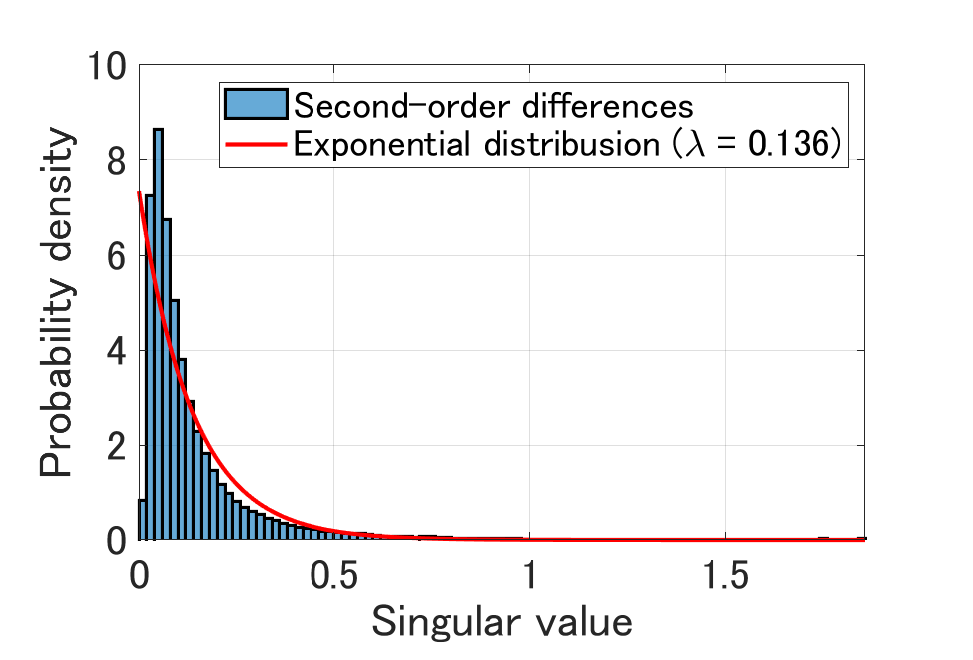
\includegraphics[width=\hsize]{./fig_supplement/Dist_Anal/SV_Dist_JasperRidge.eps}}
		\end{minipage}
		\begin{minipage}{0.325\hsize}
			\centerline{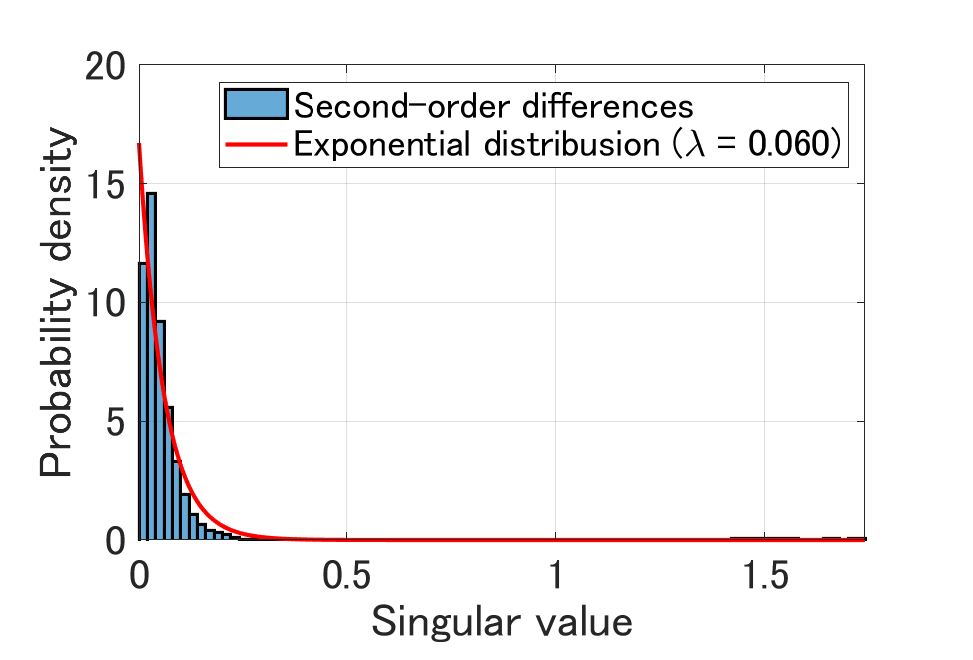
\includegraphics[width=\hsize]{./fig_supplement/Dist_Anal/SV_Dist_PaviaU120.eps}}
		\end{minipage}
		\begin{minipage}{0.325\hsize}
			\centerline{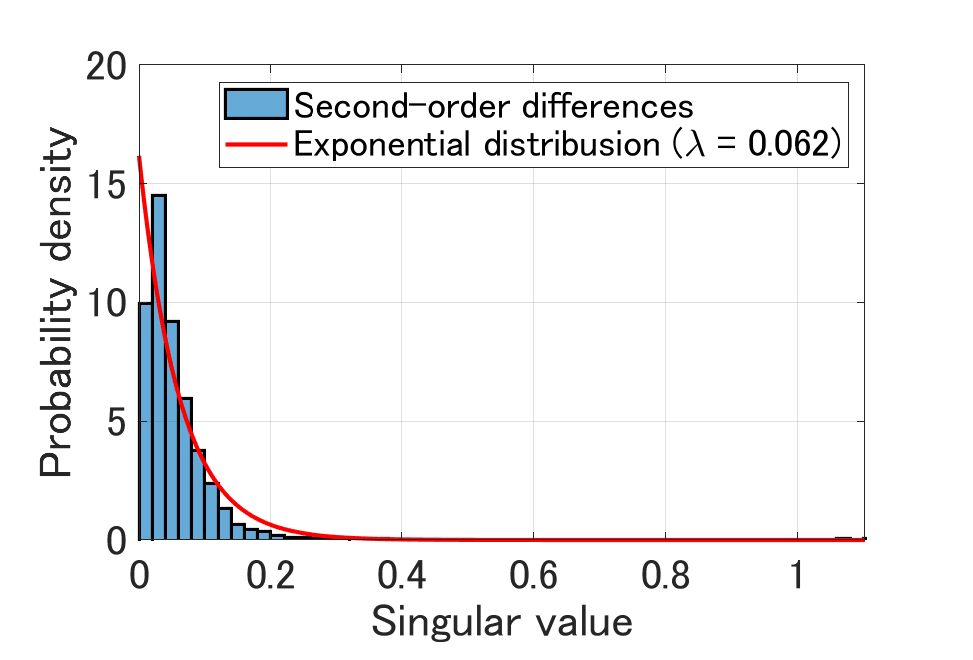
\includegraphics[width=\hsize]{./fig_supplement/Dist_Anal/SV_Dist_Beltsville.eps}}
		\end{minipage}
		
		\vspace{1mm}
		
		\begin{minipage}{0.325\hsize}
			\centerline{\small{(a)}}
		\end{minipage}
		\begin{minipage}{0.325\hsize}
			\centerline{\small{(b)}}
		\end{minipage}
		\begin{minipage}{0.325\hsize}
			\centerline{\small{(c)}}
		\end{minipage}
		
	\end{center}
	
	\caption{Normalized histograms of singular values computed from all spatio-spectral structure tensors, along with the fitted exponential distributions: (a) Jasper Ridge, (b) Pavia University, and (c) Beltsville.}
	
	\label{fig:data_dist}
\end{figure*}


\begin{table*}[t]
	\begin{center}
		\caption{MPSNRs of the Simulated HS Image Denoising Results.}
		\label{tab:MPSNR}
		\scalebox{0.70}{
			\begin{tabular}{cc cccccccccccc}
				\toprule
				Image & Noise & SSTV~\cite{Aggarwal2016SSTV} & HSSTV1~\cite{Takeyama2020HSSTV} & HSSTV2~\cite{Takeyama2020HSSTV} & $\llHTV$~\cite{Wang2021l0l1HTV} & STV~\cite{Lefkimmiatis2015STV} & SSST~\cite{Kurihara2017SSST} & LRTDTV~\cite{Wang2018LRTDTV} & FGSLR~\cite{Chen2022FGSLR} & TPTV~\cite{Chen2023TPTV} & QRNN3D~\cite{Wei2021QRNN3D} & FastHyMix~\cite{Zhuang2023FastHyMix} & $\SSSTTV$ \\
				\cmidrule(lr){1-14} 

				\multirow{8}{*}{Jasper Ridge} 
				& Case 1 & 
				36.24 & \underline{36.28} & 35.79 & 35.47 & 28.01 & 35.05 & 34.98 & 33.51 & 34.22 & 28.42 & \textbf{38.69} & 35.51 \\ 
				& Case 2 & 
				\underline{39.43} & 39.04 & 39.10 & 38.59 & 29.67 & 36.59 & 37.73 & 35.51 & 39.01 & 31.99 & 27.76 & \textbf{39.99} \\ 
				& Case 3 & 
				34.33 & 34.01 & \underline{34.83} & 34.12 & 27.07 & 32.09 & 34.75 & 33.27 & 33.74 & 27.75 & 25.56 & \textbf{36.15} \\ 
				& Case 4 & 
				42.68 & 41.54 & \underline{44.77} & 43.17 & 38.93 & 41.40 & 36.91 & 41.61 & \textbf{51.57} & 24.56 & 34.88 & 44.26 \\ 
				& Case 5 & 
				39.10 & \underline{39.31} & 38.44 & 38.96 & 30.60 & 37.67 & 35.84 & 35.49 & 37.87 & 23.95 & 35.15 & \textbf{40.04} \\ 
				& Case 6 & 
				34.22 & 34.81 & 33.97 & 34.57 & 27.95 & \underline{34.90} & 33.56 & 33.28 & 33.48 & 23.52 & 34.22 & \textbf{35.50} \\ 
				& Case 7 & 
				\underline{39.40} & 39.12 & 38.71 & 38.47 & 29.40 & 35.72 & 35.95 & 35.32 & 37.96 & 23.71 & 37.22 & \textbf{39.82} \\ 
				& Case 8 & 
				34.68 & 34.22 & \underline{35.15} & 34.27 & 26.79 & 30.99 & 33.49 & 33.07 & 33.15 & 23.22 & 23.17 & \textbf{36.05} \\ 

				\cmidrule(lr){1-14} 

				\multirow{8}{*}{Pavia University} 
				& Case 1 & 
				35.83 & \underline{36.24} & 35.39 & 35.30 & 28.33 & 35.08 & 32.79 & 32.55 & 31.52 & 31.61 & \textbf{37.69} & 35.73 \\ 
				& Case 2 & 
				38.67 & 38.55 & 38.81 & 38.20 & 29.85 & 35.40 & 35.18 & 35.40 & 37.14 & 36.38 & \underline{39.08} & \textbf{39.79} \\ 
				& Case 3 & 
				33.05 & 33.50 & 33.49 & 32.98 & 27.48 & 31.89 & 32.66 & 31.90 & 31.19 & 31.30 & \textbf{36.03} & \underline{34.39} \\ 
				& Case 4 & 
				41.34 & 40.72 & \underline{44.82} & 42.29 & 39.31 & 40.87 & 32.34 & 40.31 & \textbf{48.37} & 35.42 & 34.31 & 43.41 \\ 
				& Case 5 & 
				39.54 & \underline{39.63} & 38.89 & 39.32 & 30.74 & 36.82 & 32.47 & 35.48 & 36.08 & 34.57 & 34.78 & \textbf{40.30} \\ 
				& Case 6 & 
				34.39 & \underline{35.03} & 34.11 & 34.82 & 28.32 & 34.95 & 30.84 & 31.87 & 31.66 & 31.43 & 33.60 & \textbf{35.16} \\ 
				& Case 7 & 
				\underline{38.80} & 38.68 & 38.78 & 38.05 & 29.62 & 34.53 & 32.41 & 35.19 & 35.79 & 33.58 & 31.98 & \textbf{39.36} \\ 
				& Case 8 & 
				33.06 & 33.53 & \underline{33.62} & 32.83 & 27.22 & 30.80 & 30.84 & 31.67 & 31.13 & 30.74 & 31.79 & \textbf{34.33} \\ 

				\cmidrule(lr){1-14} 

				\multirow{8}{*}{Beltsville} 
				& Case 1 & 
				35.20 & \underline{35.89} & 34.88 & 34.71 & 28.95 & 35.79 & 34.15 & 34.58 & 32.24 & 27.91 & \textbf{39.29} & 35.35 \\ 
				& Case 2 & 
				37.87 & 38.19 & 37.66 & 37.34 & 30.66 & 36.74 & \underline{38.67} & 36.65 & 37.78 & 30.34 & 37.85 & \textbf{39.46} \\ 
				& Case 3 & 
				32.86 & 33.87 & 32.87 & 32.68 & 28.20 & 32.26 & 34.05 & \underline{34.34} & 31.75 & 27.52 & \textbf{36.00} & 34.21 \\ 
				& Case 4 & 
				41.21 & 40.88 & 41.48 & 41.56 & 37.73 & 40.18 & 38.79 & \underline{42.89} & \textbf{53.00} & 29.05 & 36.29 & 40.84 \\ 
				& Case 5 & 
				38.46 & \underline{38.75} & 38.04 & 38.16 & 30.57 & 36.98 & 33.31 & 36.55 & 36.83 & 28.88 & 35.14 & \textbf{39.71} \\ 
				& Case 6 & 
				33.92 & 34.64 & 33.74 & 34.21 & 28.47 & \underline{34.72} & 30.44 & 34.15 & 32.92 & 27.93 & 34.12 & \textbf{35.31} \\ 
				& Case 7 & 
				38.02 & \underline{38.22} & 37.66 & 37.23 & 29.87 & 35.35 & 32.76 & 36.37 & 37.09 & 28.44 & 37.13 & \textbf{38.91} \\ 
				& Case 8 & 
				33.07 & 33.92 & 33.20 & 32.65 & 27.65 & 30.82 & 30.44 & \underline{33.94} & 32.31 & 27.29 & 33.23 & \textbf{34.42} \\ 

				\bottomrule
			\end{tabular}
		}
	\end{center}
	% \vspace{-3mm}
\end{table*}
\begin{table*}[t]
	\begin{center}
		\caption{MSSIMs of the Simulated HS Image Denoising Results.}
		\label{tab:MSSIM}
		\scalebox{0.70}{
			\begin{tabular}{cc cccccccccccc}
				\toprule
				Image & Noise & SSTV~\cite{Aggarwal2016SSTV} & HSSTV1~\cite{Takeyama2020HSSTV} & HSSTV2~\cite{Takeyama2020HSSTV} & $\llHTV$~\cite{Wang2021l0l1HTV} & STV~\cite{Lefkimmiatis2015STV} & SSST~\cite{Kurihara2017SSST} & LRTDTV~\cite{Wang2018LRTDTV} & FGSLR~\cite{Chen2022FGSLR} & TPTV~\cite{Chen2023TPTV} & QRNN3D~\cite{Wei2021QRNN3D} & FastHyMix~\cite{Zhuang2023FastHyMix} & $\SSSTTV$ \\
				\cmidrule(lr){1-14} 

				\multirow{8}{*}{Jasper Ridge} 
				& Case 1 & 
				0.9266 & \underline{0.9399} & 0.9228 & 0.9063 & 0.7492 & 0.9349 & 0.9152 & 0.9172 & 0.8729 & 0.8427 & \textbf{0.9664} & 0.9121 \\ 
				& Case 2 & 
				0.9631 & \textbf{0.9660} & 0.9606 & 0.9513 & 0.8228 & 0.9518 & 0.9544 & 0.9452 & 0.9521 & 0.8951 & 0.8687 & \underline{0.9647} \\ 
				& Case 3 & 
				0.9086 & 0.9099 & \underline{0.9151} & 0.8959 & 0.7156 & 0.8779 & 0.9123 & 0.9142 & 0.8676 & 0.8235 & 0.7833 & \textbf{0.9266} \\ 
				& Case 4 & 
				0.9823 & 0.9783 & 0.9823 & 0.9826 & 0.9740 & 0.9803 & 0.9572 & 0.9836 & \textbf{0.9895} & 0.8587 & 0.9106 & \underline{0.9838} \\ 
				& Case 5 & 
				0.9570 & \underline{0.9638} & 0.9522 & 0.9525 & 0.8433 & 0.9613 & 0.9316 & 0.9436 & 0.9370 & 0.8389 & 0.9051 & \textbf{0.9648} \\ 
				& Case 6 & 
				0.8854 & 0.9090 & 0.8829 & 0.8879 & 0.7448 & \textbf{0.9328} & 0.8787 & 0.9106 & 0.8574 & 0.7946 & 0.8900 & \underline{0.9131} \\ 
				& Case 7 & 
				0.9625 & \textbf{0.9662} & 0.9569 & 0.9494 & 0.8146 & 0.9426 & 0.9326 & 0.9423 & 0.9451 & 0.8290 & 0.9509 & \underline{0.9641} \\ 
				& Case 8 & 
				0.9129 & 0.9136 & \underline{0.9183} & 0.8958 & 0.7050 & 0.8484 & 0.8807 & 0.9084 & 0.8530 & 0.7787 & 0.6000 & \textbf{0.9257} \\ 

				\cmidrule(lr){1-14} 

				\multirow{8}{*}{Pavia University} 
				& Case 1 & 
				0.9254 & \underline{0.9389} & 0.9171 & 0.9145 & 0.7182 & 0.9269 & 0.8650 & 0.9034 & 0.8120 & 0.9111 & \textbf{0.9558} & 0.9204 \\ 
				& Case 2 & 
				0.9599 & 0.9616 & 0.9586 & 0.9544 & 0.7902 & 0.9345 & 0.9196 & 0.9436 & 0.9399 & 0.9599 & \textbf{0.9723} & \underline{0.9669} \\ 
				& Case 3 & 
				0.8784 & 0.8915 & 0.8848 & 0.8761 & 0.6766 & 0.8582 & 0.8624 & 0.8846 & 0.8071 & 0.9027 & \textbf{0.9470} & \underline{0.9041} \\ 
				& Case 4 & 
				0.9762 & 0.9742 & \textbf{0.9853} & 0.9784 & 0.9727 & 0.9771 & 0.9077 & 0.9822 & 0.9754 & 0.9570 & 0.9337 & \underline{0.9850} \\ 
				& Case 5 & 
				0.9657 & \underline{0.9689} & 0.9596 & 0.9626 & 0.8202 & 0.9477 & 0.8808 & 0.9445 & 0.9216 & 0.9475 & 0.9180 & \textbf{0.9704} \\ 
				& Case 6 & 
				0.8980 & \underline{0.9177} & 0.8915 & 0.9049 & 0.7192 & \textbf{0.9254} & 0.8137 & 0.8976 & 0.8193 & 0.9068 & 0.8968 & 0.9112 \\ 
				& Case 7 & 
				0.9612 & \underline{0.9629} & 0.9587 & 0.9532 & 0.7826 & 0.9207 & 0.8778 & 0.9414 & 0.9221 & 0.9343 & 0.9132 & \textbf{0.9647} \\ 
				& Case 8 & 
				0.8788 & \underline{0.8923} & 0.8869 & 0.8731 & 0.6649 & 0.8210 & 0.8127 & 0.8807 & 0.8068 & 0.8900 & 0.8726 & \textbf{0.9029} \\ 

				\cmidrule(lr){1-14} 

				\multirow{8}{*}{Beltsville} 
				& Case 1 & 
				0.9121 & 0.9310 & 0.9058 & 0.9004 & 0.7256 & \underline{0.9328} & 0.8776 & 0.9131 & 0.8172 & 0.8404 & \textbf{0.9641} & 0.9075 \\ 
				& Case 2 & 
				0.9510 & 0.9566 & 0.9474 & 0.9442 & 0.7994 & 0.9412 & 0.9512 & 0.9483 & 0.9425 & 0.8905 & \textbf{0.9665} & \underline{0.9618} \\ 
				& Case 3 & 
				0.8712 & 0.8941 & 0.8696 & 0.8700 & 0.6870 & 0.8633 & 0.8772 & \underline{0.9090} & 0.8064 & 0.8270 & \textbf{0.9455} & 0.8986 \\ 
				& Case 4 & 
				0.9728 & 0.9729 & 0.9728 & 0.9730 & 0.9556 & 0.9713 & 0.9579 & \textbf{0.9832} & \underline{0.9823} & 0.8837 & 0.9440 & 0.9721 \\ 
				& Case 5 & 
				0.9540 & \underline{0.9605} & 0.9491 & 0.9508 & 0.7987 & 0.9462 & 0.8889 & 0.9484 & 0.9327 & 0.8755 & 0.9165 & \textbf{0.9648} \\ 
				& Case 6 & 
				0.8807 & 0.9056 & 0.8759 & 0.8878 & 0.7044 & \textbf{0.9187} & 0.7900 & 0.9094 & 0.8432 & 0.8471 & 0.8956 & \underline{0.9101} \\ 
				& Case 7 & 
				0.9526 & \underline{0.9582} & 0.9475 & 0.9435 & 0.7717 & 0.9249 & 0.8862 & 0.9462 & 0.9325 & 0.8655 & 0.9542 & \textbf{0.9592} \\ 
				& Case 8 & 
				0.8757 & 0.8967 & 0.8767 & 0.8687 & 0.6586 & 0.8255 & 0.7891 & \textbf{0.9053} & 0.8268 & 0.8250 & 0.9017 & \underline{0.9021} \\ 

				\bottomrule
				
			\end{tabular}
		}
	\end{center}
	% \vspace{-3mm}
\end{table*}

